\documentclass[12pt]{beamer}

\usepackage{amsmath}
\usepackage{amsfonts}
\usepackage{pgfplots}
\pgfplotsset{compat=1.18}

\usetheme{Berlin}
\usecolortheme{default}
\usefonttheme{serif}

\setbeamertemplate{navigation symbols}{}
% \setbeamercovered{transparent}
% \setbeameroption{show notes on second screen}

\DeclareMathOperator{\proj}{proj}

\title{Orthogonal Projection}
\author{Alvin Kim}
% \institute{Math Kimchi}
\logo{
\includegraphics[height=0.7cm]{../mathkimchi.jpg} \hspace{0.5em}}

\begin{document}

\begin{frame}
    \titlepage
\end{frame}

\begin{frame}[allowframebreaks]
    \begin{columns}
        \column{0.5\textwidth}
        \tableofcontents[sections={1-3}]

        \column{0.5\textwidth}
        \tableofcontents[sections={4-}]
    \end{columns}
\end{frame}

\section{Introduction}

\subsection{Definitions}

\begin{frame}
    \frametitle{What is a projection?}
    $\proj_S \vec{b}$, the projection of vector $\vec{b}$ onto subspace $S$, is the vector inside of $S$ closest to $\vec{b}$.

    \only<2>{
        \begin{block}{Note}
            In this presentation, projection refers to specifically orthogonal projection, $\vec{p}$ refers to $\proj_S \vec{b}$, and $\vec{e}$ refers to the error vector $\vec{e} = \vec{b} - \vec{p}$.
            The error vector is also called the rejection.
        \end{block}
    }

    \only<3->{
        Closest means that the error is orthogonal to $S$.

        \note{The reason why I am using this meaning rather than the minimizing error meaning is because this meaning is simpler to work with. Ultimately, it can be proven that both meanings are the same.}
    }

    \only<4>{
        \begin{block}{Note}
            The dimension of subspace S can be anything from 0 to the dimension of the space we are working inside.
        \end{block}
    }
\end{frame}

\subsection{Example}
\begin{frame}
    \frametitle{Example}

    \begin{columns}
        \column{0.5\textwidth}
        \begin{center}
            \begin{tikzpicture}[scale=0.5]
                \draw[very thin,gray] (-4,-4) grid (4,4);
                \draw[->] (-4,0)--(4.5,0) node[right]{$x$};
                \draw[->] (0,-4)--(0,4.5) node[above]{$y$};
                \only<2->{\draw[-,dashed,gray] (-3.99,-1.33)--(4.5,1.5) node[below]{$S$};}
                \draw[->,red,thick] (0,0)--(3,1) node[below]{$\vec{a}$};
                \draw[->,blue,thick] (0,0)--(-3,2) node[left]{$\vec{b}$};
                \only<3->{\draw[->,green,thick] (0,0)--(-2.1,-0.7) node[below]{$\vec{p}$};}
                \only<4->{\draw[-,gray] (-3,2)--(-2.1,-0.7) node[left,midway]{$\vec{e}$};}
            \end{tikzpicture}
        \end{center}
        \column{0.5\textwidth}
        \only<1> {
            \begin{example}
                Draw $\proj_a b$.
            \end{example}
        }
        \only<2>{
            \begin{block}{Note}
                When projecting a vector onto another vector $\vec{a}$, the subspace $S$ is the span of $\vec{a}$.
            \end{block}
        }
    \end{columns}
\end{frame}

\section{Formulas}

\subsection{Projection onto a Vector}

\begin{frame}
    \frametitle{Projection onto a Vector}

    \begin{columns}
        \column{0.5\textwidth}
        Consider projecting $\vec{b}$ onto $\vec{a}$.

        \note{If $\vec{a}=\vec{0}$, then p will be 0 because p must be in the zero subspace. If $\vec{a}\neq 0$, then we are projecting b onto the line that spans $\vec{a}$.}

        \pause

        What we know:
        \begin{align*}
            \vec{e} = \vec{b} - \vec{p} \\
            \vec{p} = c \vec{a}         \\
            \vec{e} \cdot \vec{a} = 0
        \end{align*}

        \column{0.5\textwidth}
        \note{tell the audience to try this}

        \pause
        From that:
        \begin{align*}
            \alert<+>{\vec{e} = \vec{b} - c \vec{a}                          } \\
            \alert<+>{(\vec{b} - c \vec{a}) \cdot \vec{a} = 0                } \\
            \alert<+>{\vec{b} \cdot \vec{a} - c \vec{a} \cdot \vec{a} = 0    } \\
            \alert<+>{\vec{b} \cdot \vec{a} = c \vec{a} \cdot \vec{a}        } \\
            \alert<+>{c = \frac{\vec{a} \cdot \vec{b}}{\vec{a} \cdot \vec{a}}} \\
            \alert<+>{\boxed{\vec{p} = \frac{\vec{a} \cdot \vec{b}}{\vec{a} \cdot \vec{a}} \vec{a}}}
        \end{align*}
    \end{columns}
\end{frame}

\subsection{Projection onto a Subspace}

\begin{frame}
    \frametitle{Project $\vec{b}$ onto $S$}

    \begin{columns}
        \column{0.6\textwidth}
        \pause

        Suppose that $\vec{a}_1, \vec{a}_2, \dots, \vec{a}_n$ are a basis of $S$, let
        $$
            A =
            \begin{bmatrix}
                \vert     & \vert     &        & \vert     \\
                \vec{a}_1 & \vec{a}_2 & \hdots & \vec{a}_n \\
                \vert     & \vert     &        & \vert     \\
            \end{bmatrix}
        $$
        \note{the a vecs are LI, but the A matrix might be rectangular so it isn't invertable}
        and let $\vec{p} = A\vec{c}$.
        \note{there is guranteed to be exactly one c for a specific p and A bc p is in S and A has LI cols}
        We also know:
        \begin{align*}
            \vec{e} = \vec{b} - \vec{p} \\
            \alt<+>{C(A)^\perp = N(A^T)}{A^T \vec{e} = \vec{0}} \note{the orthogonal complement of col space is the left null space}
        \end{align*}

        \column{0.4\textwidth}
        \note{tell them to try this proof}
        \note{Hint: ATA is invertible bc A has LI columns}
        \pause
        Then,
        \begin{align*}
            \vec{e} = \vec{b} - A\vec{c}               \\
            A^T (\vec{b} - A\vec{c}) = \vec{0}         \\
            A^T \vec{b} - A^T A \vec{c} = \vec{0}      \\
            A^T \vec{b} = A^T A \vec{c}                \\
            (A^T A)^{-1} A^T \vec{b} = \vec{c}         \\
            \boxed{\vec{c} = (A^T A)^{-1} A^T \vec{b}} \\
            \boxed{\vec{p} = A(A^T A)^{-1} A^T \vec{b}}
        \end{align*}

        \note{the coefficients vector is also good to remember, because it is sometimes more useful than the projection}
        \note{as mentioned before, we can't distribute the inverse sign because A might be rectangular}
    \end{columns}
\end{frame}

\subsection{The Projection Matrix}

\begin{frame}
    \frametitle{The Projection Matrix}

    Recall that for some matrix $A$, the projection $\vec{p} = A(A^T A)^{-1} A^T \vec{b}$.

    \only<+>{
        \begin{block}{Observation}
            For a specific $A$, $\vec{p}$ is an unchanging linear transformation of $\vec{b}$.
            So, we can represent the linear transformation with a matrix $P$.
            \note{To multiply some vector by a matrix is to apply a linear transformation to the vector.}
        \end{block}
    }

    \pause

    Let $\boxed{P = A(A^T A)^{-1} A^T}$.
    Then, $\vec{p} = P \vec{b}$.

    \only<+>{
        \begin{alertblock}{Note}
            $A$ must have linearly independent columns.
        \end{alertblock}
    }
\end{frame}

\subsection{The Error Matrix}

\begin{frame}
    \frametitle{The Error Matrix}

    The error vector is $\vec{b}$ projected onto $S^\perp$.
    \pause
    Since finding the error vector is also a projection, there should be an error matrix $E$ for some $P$ such that $\vec{e} = E\vec{b}$.
    \pause
    \begin{align*}
        \vec{e} = \vec{b} - \vec{p}     \\
        \vec{e} = I \vec{b} - P \vec{b} \\
        \vec{e} = (I - P) \vec{b}       \\
        \boxed{E = I - P}
    \end{align*}
\end{frame}

\section{Properties}

\subsection{Projection Minimizes Error}

\subsection{$P^T$}

\subsection{$P^2$}

\subsection{Sanity Check: $E^2$}

\section{Special Cases}

\subsection{Sanity Check: $A$ Has One Column}

\subsection{Projection from $\boldmath{R}^3$ onto y-axis}

\subsection{Projection from $\boldmath{R}^3$ onto xz-plane}

\subsection{$A$ is an Orthonormal Matrix}

\subsection{$\vec{b} \perp S$}

\subsection{$\vec{b} \in S$}

\section{Conclusion}

\subsection{Formulas Recapped}

\subsection{Properties Recapped}

\subsection{Conclusion}

\begin{frame}
    \begin{itemize}
        \item Applications
              \begin{itemize}
                  \item Graphics
                  \item Least Squares Regression
              \end{itemize}
        \item Further Learning
              \begin{itemize}
                  \item Practice
                  \item \textit{Introduction to Linear Algebra} 6th Edition Chapter 4.2 by Gilbert Strang
              \end{itemize}
    \end{itemize}
\end{frame}

\end{document}